\section{Конструкторский раздел}

В данном разделе будет представлена схема проектируемой базы данных, будут описаны сущности базы данных, ограничения целостности, ролевая модель и используемые функции, процедуры и триггеры.

\subsection{Проектирование базы данных}

На рисунке \ref{fig:erd} представлена схема проектируемой базы данных.

\begin{figure}[H]
	\centering
	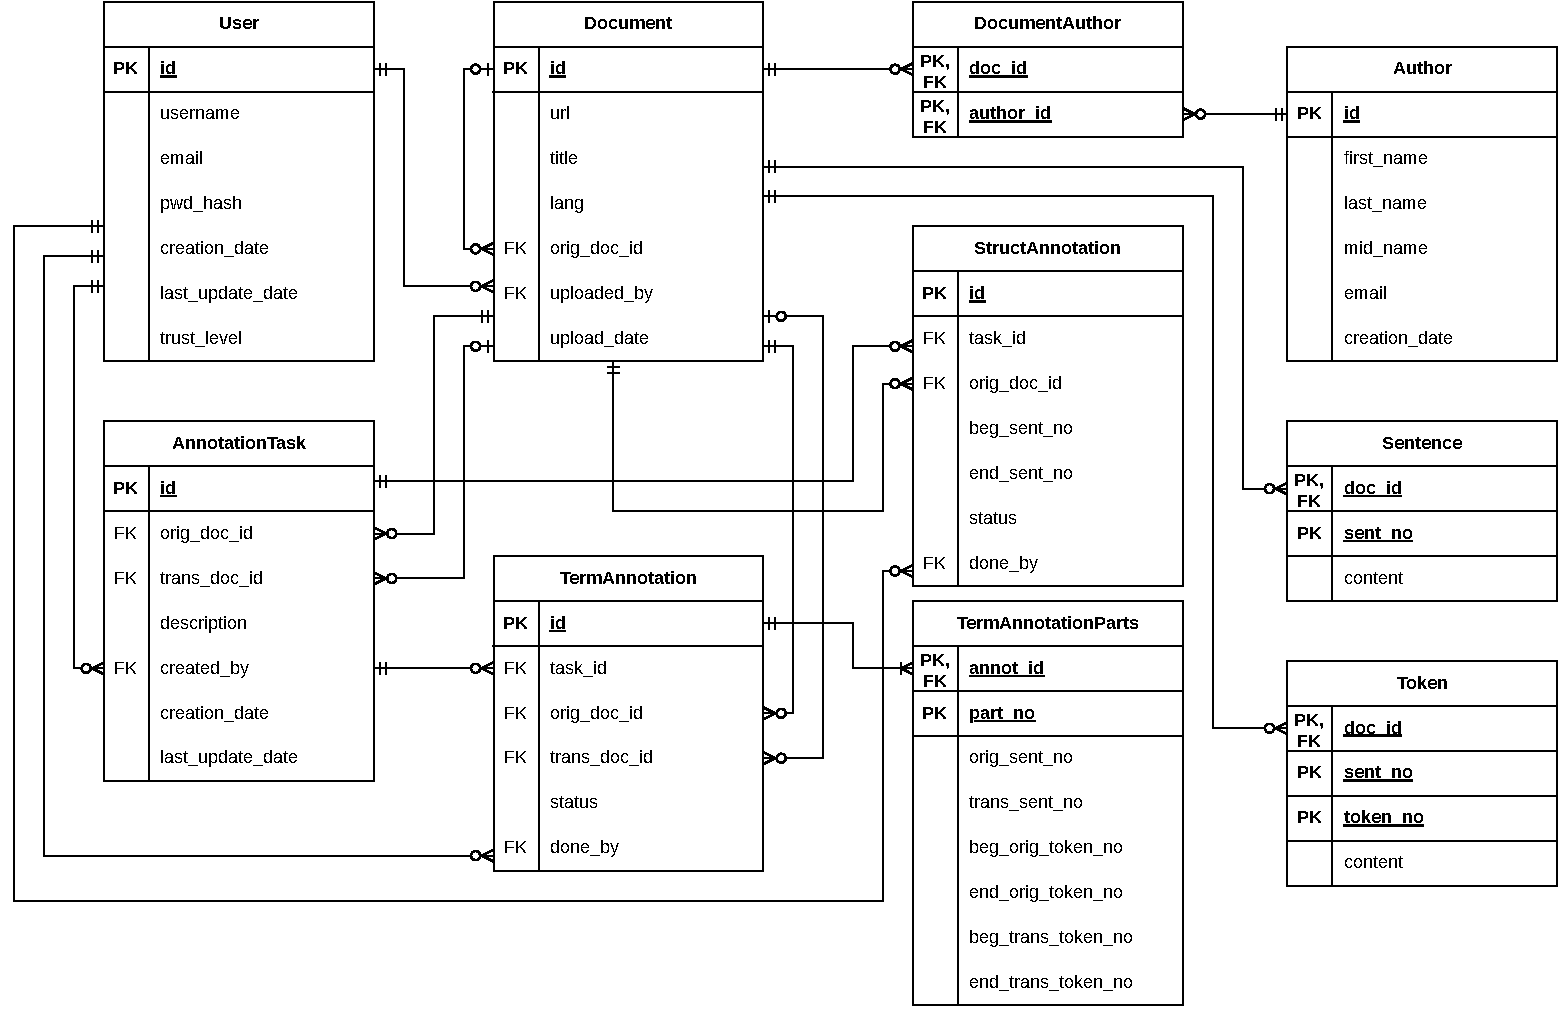
\includegraphics[width=\textwidth]{diag/erd-v3.pdf}
	% 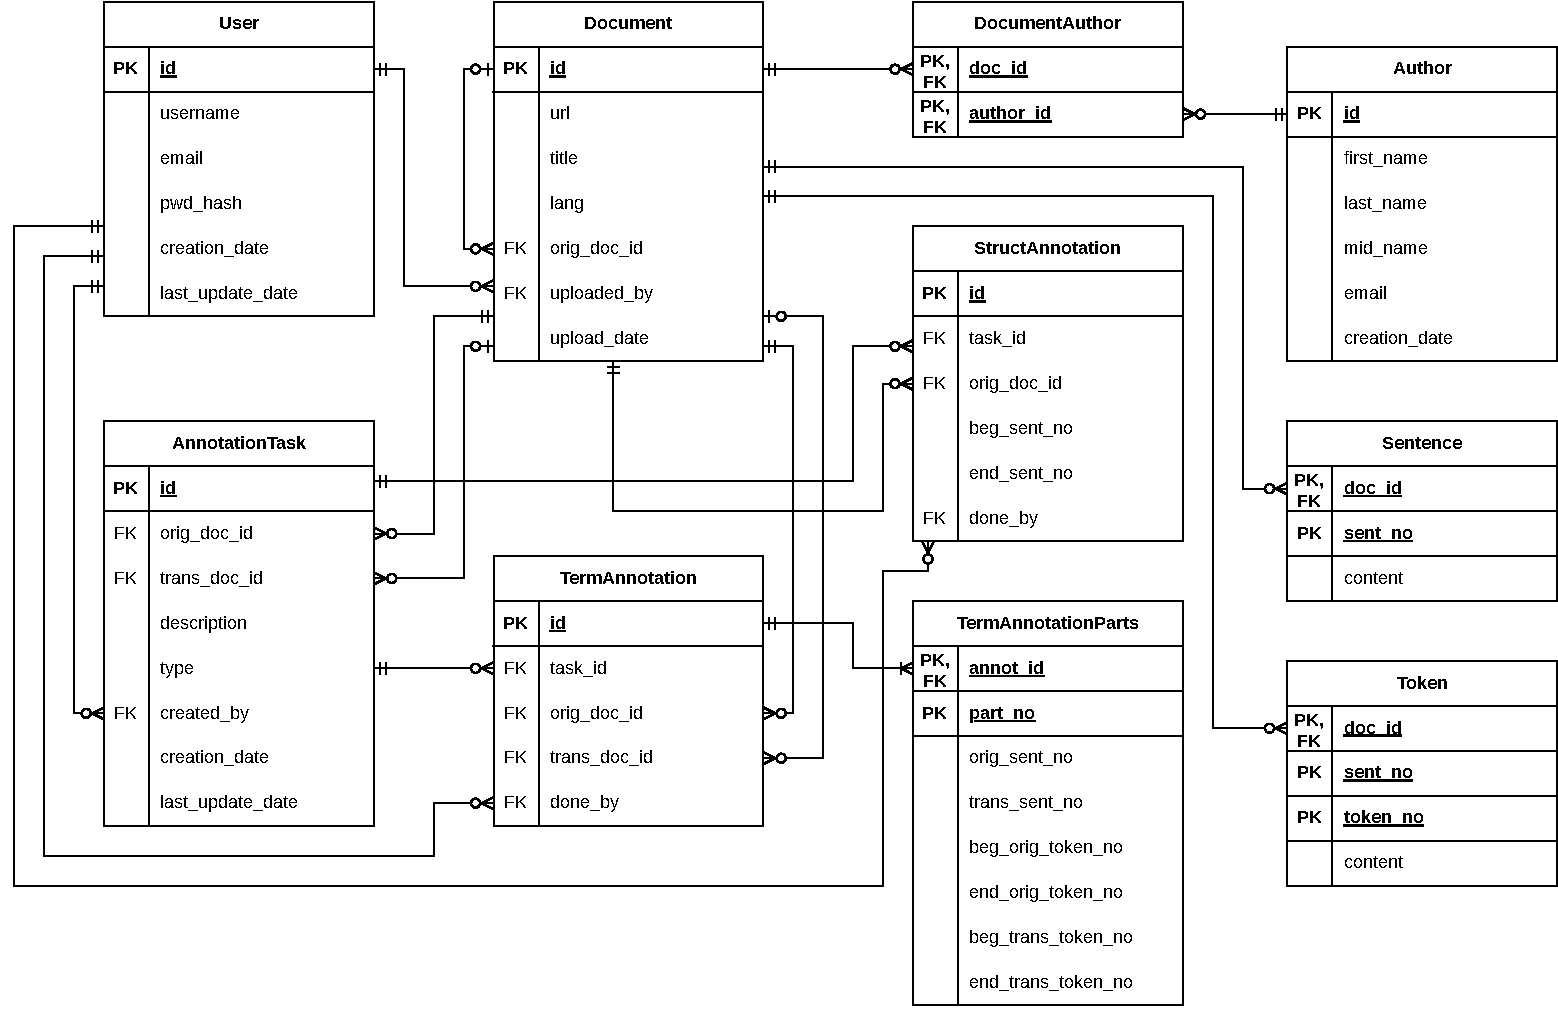
\includegraphics[angle=90, width=0.75\textwidth]{diag/crow-foot-erd.pdf}
	\caption{ER-диаграмма проектируемой базы данных в нотации Мартина}
	\label{fig:erd}
\end{figure}

\subsection{Описание сущностей}

В данном подразделе будут описаны десять сущностей проектируемой базы данных: User, Document, DocumentAuthor, Author, AnnotationTask, Struct-Annotation, TermAnnotation, TermAnnotationPart, Sentence, Token.

\subsubsection*{User}

Сущность User формализует пользователя базы данных и имеет следующие поля:
\begin{itemize}
    \item id --- идентификатор пользователя;
    \item username --- имя пользователя;
    \item email --- электронная почта пользователя;
    \item pwd\_hash --- хеш пароля пользователя;
    \item trust\_level --- уровень доверия пользователя (зависит от качества и количества совершенных разметок);
    \item creation\_date --- дата регистрации пользователя;
    \item last\_update\_date --- дата последнего обновления информации о пользователе.
\end{itemize}

\subsubsection*{Document}

Сущность Document формализует документ, хранимый в корпусе, и имеет следующие поля:
\begin{itemize}
    \item id --- идентификатор документа;
    \item url --- ссылка на документ (в сети или файловой системе);
    \item title --- название документа / статьи;
    \item lang --- язык документа;
    \item orig\_doc\_id --- ссылка на оригинальный документ, в случае, если данный документ является переводом;
    \item uploaded\_by --- ссылка на пользователя, загрузившего документ в систему;
    \item upload\_date --- дата загрузки документа в систему.
\end{itemize}

\subsubsection*{DocumentAuthor}

Сущность DocumentAuthor формализует связь <<многие-ко-многим>> документов и авторов:
\begin{itemize}
    \item doc\_id --- идентификатор документа;
    \item author\_id --- идентификатор автора документа.
\end{itemize}

\subsubsection*{Author}

Сущность Author формализует автора документов:
\begin{itemize}
    \item id --- идентификатор автора;
    \item first\_name --- имя автора;
    \item last\_name --- фамилия автора;
    \item mid\_name --- отчество автора;
    \item email --- электронная почта автора;
    \item creation\_date --- дата появления сущности в системе.
\end{itemize}

\subsubsection*{AnnotationTask}

Сущность AnnotationTask формализует задание на разметку:
\begin{itemize}
    \item id --- идентификатор задания на разметку;
    \item orig\_doc\_id --- ссылка на оригинальный документ, участвующий в разметке;
    \item trans\_doc\_id --- ссылка на перевод документа, участвующий в разметке;
    \item description --- описание задания на разметку;
    \item created\_by --- ссылка на пользователя, создавшего задание на разметку;
    \item creation\_date --- дата создания задания на разметку;
    \item last\_update\_date --- дата последнего обновления задания на разметку.
\end{itemize}

\subsubsection*{StructAnnotation}

Сущность StructAnnotation формализует структурную разметку:
\begin{itemize}
    \item id --- идентификатор структурной разметки;
    \item task\_id --- ссылка на задание на разметку, результатом выполнения которого данная разметка является;
    \item orig\_doc\_id --- ссылка на документ, для которого выполняется структурная разметка;
    \item beg\_sent\_no --- номер начального предложения разметки;
    \item end\_sent\_no --- номер последнего предложения разметки;
    \item status --- статус разметки (утверждена модератором или нет);
    \item done\_by --- ссылка на пользователя, выполнившего разметку.
\end{itemize}

\subsubsection*{TermAnnotation}

Сущность TermAnnotation формализует терминологическую разметку:
\begin{itemize}
    \item id --- идентификатор терминологической разметки;
    \item task\_id --- ссылка на задание на разметку, результатом выполнения которого данная разметка является;
    \item orig\_doc\_id --- ссылка на оригинальный документ, для которого выполняется терминологическая разметка;
    \item trans\_doc\_id --- ссылка на перевод документа, для которого выполняется терминологическая разметка;
    \item status --- статус разметки (утверждена модератором или нет);
    \item done\_by --- ссылка на пользователя, выполнившего разметку.
\end{itemize}

\subsubsection*{TermAnnotationPart}

Сущность TermAnnotationPart формализует составляющие терминологической разметки --- определяет границы терминов, входящих в разметку, и устанавливает их соответствие в оригинальном документе и его переводе:
\begin{itemize}
    \item annot\_id --- ссылка на идентификатор терминологической разметки;
    \item part\_no --- номер части, термина, входящего в терминологическую разметку;
    \item orig\_sent\_no --- номер предложения в оригинальном документе;
    \item trans\_sent\_no --- номер предложения в документе-переводе;
    \item beg\_orig\_token\_no --- номер токена, являющегося началом термина в оригинальном документе;
    \item end\_orig\_token\_no --- номер токена, являющегося концом термина в оригинальном документе;
    \item beg\_trans\_token\_no --- номер токена, являющегося началом термина в документе-переводе;
    \item end\_trans\_token\_no --- номер токена, являющегося концом термина в документе-переводе.
\end{itemize}

\subsubsection*{Sentence}

Сущность Sentence формализует предложение текста документа:
\begin{itemize}
    \item doc\_id --- ссылка на документ, к которому относится предложение;
    \item sent\_no --- номер предложения в документе;
    \item content --- текст предложения.
\end{itemize}

\subsubsection*{Token}

Сущность Token формализует токен, получаемый в процессе токенизации текста документа:
\begin{itemize}
    \item doc\_id --- ссылка на документ, в котором содержится предложение, которому принадлежит токен;
    \item sent\_no --- номер предложения в документе, которому принадлежит токен;
    \item token\_no --- номер токена в предложении;
    \item content --- текст токена.
\end{itemize}

\subsection{Описание ограничений целостности}

В данном подразделе в таблицах \ref{tab:user} -- \ref{tab:token} будут описаны проектируемые ограничения целостности базы данных в контексте выбранной, реляционной, модели.

\begin{table}[H]
\centering
\caption{Ограничение целостности User}
\begin{tabular}{|m{4cm}|m{3cm}|m{6cm}|}
\hline
\textbf{Поле} & \textbf{Тип} & \textbf{Ограничение} \\ \hline
id & UUID & первичный ключ \\ \hline
username & строка & уникальный, не пустое значение \\ \hline
email & строка & не пустое значение \\ \hline
pwd\_hash & строка & не пустое значение \\ \hline
trust\_level & вещественное число & не пустое значение, по умолчанию 0 \\ \hline
creation\_date & временная метка & не пустое значение \\ \hline
last\_update\_date & временная метка & не пустое значение \\ \hline
\end{tabular}
\label{tab:user}
\end{table}

\begin{table}[H]
\centering
\caption{Ограничение целостности Document}
\begin{tabular}{|m{3cm}|m{3cm}|m{6cm}|}
\hline
\textbf{Поле} & \textbf{Тип} & \textbf{Ограничение} \\ \hline
id & UUID & первичный ключ \\ \hline
url & строка & не пустое значение \\ \hline
title & строка & не пустое значение \\ \hline
lang & строка & не пустое значение \\ \hline
orig\_doc\_id & UUID & внешний ключ на поле id таблицы Document \\ \hline
uploaded\_by & UUID & внешний ключ на поле id таблицы User, не пустое значение \\ \hline
upload\_date & временная метка & не пустое значение \\ \hline
\end{tabular}
\label{tab:doc}
\end{table}

\begin{table}[H]
\centering
\caption{Ограничение целостности DocumentAuthor}
\begin{tabular}{|m{3cm}|m{3cm}|m{6cm}|}
\hline
\textbf{Поле} & \textbf{Тип} & \textbf{Ограничение} \\ \hline
doc\_id & UUID & первичный ключ, внешний ключ на поле id таблицы Document \\ \hline
author\_id & UUID & первичный ключ, внешний ключ на поле id таблицы Author \\ \hline
\end{tabular}
\label{tab:docauthor}
\end{table}

\begin{table}[H]
\centering
\caption{Ограничение целостности Author}
\begin{tabular}{|m{3cm}|m{3cm}|m{6cm}|}
\hline
\textbf{Поле} & \textbf{Тип} & \textbf{Ограничение} \\ \hline
id & UUID & первичный ключ \\ \hline
first\_name & строка & --- \\ \hline
last\_name & строка & --- \\ \hline
mid\_name & строка & --- \\ \hline
email & строка & --- \\ \hline
creation\_date & временная метка & не пустое значение \\ \hline
\end{tabular}
\label{tab:author}
\end{table}

\begin{table}[H]
\centering
\caption{Ограничение целостности AnnotationTask}
\begin{tabular}{|m{4cm}|m{3cm}|m{6cm}|}
\hline
\textbf{Поле} & \textbf{Тип} & \textbf{Ограничение} \\ \hline
id & UUID & первичный ключ \\ \hline
orig\_doc\_id & UUID & внешний ключ на поле id таблицы Document, не пустое значение \\ \hline
trans\_doc\_id & UUID & внешний ключ на поле id таблицы Document \\ \hline
description & строка & не пустое значение \\ \hline
created\_by & UUID & внешний ключ на поле id таблицы User \\ \hline
creation\_date & временная метка & не пустое значение \\ \hline
last\_update\_date & временная метка & не пустое значение \\ \hline
\end{tabular}
\label{tab:annottask}
\end{table}

\begin{table}[H]
\centering
\caption{Ограничение целостности StructAnnotation}
\begin{tabular}{|m{3cm}|m{3cm}|m{6cm}|}
\hline
\textbf{Поле} & \textbf{Тип} & \textbf{Ограничение} \\ \hline
id & UUID & первичный ключ \\ \hline
task\_id & UUID & внешний ключ на поле id таблицы AnnotationTask, не пустое значение \\ \hline
orig\_doc\_id & UUID & внешний ключ на поле id таблицы Document, не пустое значение \\ \hline
beg\_sent\_no & целое число & не пустое значение \\ \hline
end\_sent\_no & целое число & не пустое значение \\ \hline
status & строка & --- \\ \hline
done\_by & UUID & внешний ключ на поле id таблицы User, не пустое значение \\ \hline
\end{tabular}
\label{tab:structannot}
\end{table}

\begin{table}[H]
\centering
\caption{Ограничение целостности TermAnnotation}
\begin{tabular}{|m{3cm}|m{3cm}|m{6cm}|}
\hline
\textbf{Поле} & \textbf{Тип} & \textbf{Ограничение} \\ \hline
id & UUID & первичный ключ \\ \hline
task\_id & UUID & внешний ключ на поле id таблицы AnnotationTask, не пустое значение \\ \hline
orig\_doc\_id & UUID & внешний ключ на поле id таблицы Document, не пустое значение \\ \hline
trans\_doc\_id & UUID & внешний ключ на поле id таблицы Document \\ \hline
status & строка & --- \\ \hline
done\_by & UUID & внешний ключ на поле id таблицы User, не пустое значение \\ \hline
\end{tabular}
\label{tab:termannot}
\end{table}

\begin{table}[H]
\centering
\caption{Ограничение целостности TermAnnotationPart}
\begin{tabular}{|m{5cm}|m{3cm}|m{6cm}|}
\hline
\textbf{Поле} & \textbf{Тип} & \textbf{Ограничение} \\ \hline
annot\_id & UUID & первичный ключ, внешний ключ на поле id таблицы TermAnnotation \\ \hline
part\_no & целое число & первичный ключ \\ \hline
orig\_sent\_no & целое число & не пустое значение \\ \hline
trans\_sent\_no & целое число & не пустое значение \\ \hline
beg\_orig\_token\_no & целое число & не пустое значение \\ \hline
end\_orig\_token\_no & целое число & не пустое значение \\ \hline
beg\_trans\_token\_no & целое число & не пустое значение \\ \hline
end\_trans\_token\_no & целое число & не пустое значение \\ \hline
\end{tabular}
\label{tab:termannotparts}
\end{table}

\begin{table}[H]
\centering
\caption{Ограничение целостности Sentence}
\begin{tabular}{|m{3cm}|m{3cm}|m{6cm}|}
\hline
\textbf{Поле} & \textbf{Тип} & \textbf{Ограничение} \\ \hline
doc\_id & UUID & первичный ключ, внешний ключ на поле id таблицы Document \\ \hline
sent\_no & целое число & первичный ключ \\ \hline
content & строка & не пустое значение \\ \hline
\end{tabular}
\label{tab:sent}
\end{table}

\begin{table}[H]
\centering
\caption{Ограничение целостности Token}
\begin{tabular}{|m{3cm}|m{3cm}|m{6cm}|}
\hline
\textbf{Поле} & \textbf{Тип} & \textbf{Ограничение} \\ \hline
doc\_id & UUID & первичный ключ, внешний ключ на поле id таблицы Document \\ \hline
sent\_no & целое число & первичный ключ \\ \hline
token\_no & целое число & первичный ключ \\ \hline
content & строка & не пустое значение \\ \hline
\end{tabular}
\label{tab:token}
\end{table}

\subsection{Описание функций, процедур и триггеров}

Чем больше пользователь производит корректных разметок, тем сильнее модераторы могут его разметкам <<доверять>>.
Рейтинг доверия пользователей можно вычислять разными способами.
Одним из примитивных способов вычисления рейтинга доверия пользователя может быть следующий: увеличивать рейтинг доверия пользователя на пять за каждую утвержденную разметку, и уменьшать на четыре --- за каждую отклоненную.
Пересчет рейтинга доверия пользователей можно производить автоматически, после проверки модератором его разметки, с помощью триггера.
Алгоритм работы триггера, срабатывающего в ответ на обновление статуса разметки, приведен на рисунке \ref{fig:trig} ниже.

\begin{figure}[H]
	\centering
	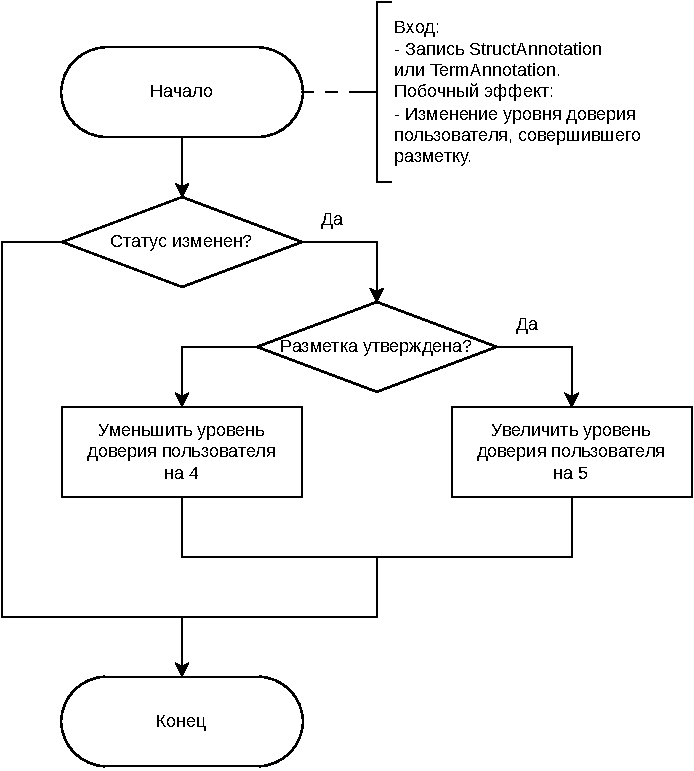
\includegraphics[width=0.7\textwidth]{diag/trig-v3.pdf}
	\caption{Схема алгоритма работы триггера, отвечающего за пересчет уровня доверия пользователей}
	\label{fig:trig}
\end{figure}

\subsection{Описание ролевой модели}

В разрабатываемой базе данных будет использоваться следующая ролевая модель:
\begin{enumerate}
    \item Пользователь --- имеет права доступа INSERT к таблицам TermAnnotation, TermAnnotationPart и StructAnnotation, права доступа SELECT к таблицам AnnotationTask, Sentence и Token.
    \item Модератор --- имеет все права доступа пользователя, а также INSERT к таблице AnnotationTask, UPDATE к таблицам AnnotationTask, Term-Annotation и StructAnnotation.
    \item Администратор --- имеет все права доступа ко всем таблицам.
\end{enumerate}

\subsection*{Вывод}

В данном разделе была представлена схема проектируемой базы данных, были описаны сущности базы данных, ограничения целостности, используемый триггер и используемая ролевая модель.
